\documentclass{article}
\usepackage[english,greek, main=greek]{babel}
\usepackage[utf8]{inputenc}
\usepackage{fullpage}
\usepackage{amsmath} 
\usepackage{graphicx} % for graphics and plots
\usepackage{subcaption} % for subfigures and subcaptions and \ContinuedFloat
\usepackage{placeins} % for \FloatBarrier
\usepackage{xcolor} % for colour definitions
\usepackage{listings} % for code highlighting
\usepackage{verbatim} % for file input
\usepackage{hyperref} % clickable links
\usepackage[explicit]{titlesec} % number after section name
\titleformat{\section}  % avoid numbering the table of contents
  {\normalfont\Large\bfseries}
  {}
  {0em}
  {\ifnum\value{section}=0\relax #1\else #1\ \thesection\fi}

\newcommand{\eng}[1]{\foreignlanguage{english}{#1}} % shortcut for inserting english into greek text

\useshorthands{;}
\defineshorthand{;}{?} % greek question mark instead of english semicolon

\definecolor{mGreen}{rgb}{0,0.6,0}
\definecolor{mGray}{rgb}{0.5,0.5,0.5}
\definecolor{mPurple}{rgb}{0.58,0,0.82}
\definecolor{light-gray}{gray}{0.95}
\definecolor{backgroundColour}{rgb}{0.95,0.95,0.92}

\lstdefinestyle{CStyle}{
    backgroundcolor=\color{backgroundColour},   
    commentstyle=\color{mGreen},
    keywordstyle=\color{magenta},
    numberstyle=\tiny\color{mGray},
    stringstyle=\color{mPurple},
    basicstyle=\footnotesize,
    breakatwhitespace=false,         
    breaklines=true,                 
    keepspaces=true,                 
    numbers=left,                    
    numbersep=5pt,                  
    showspaces=false,                
    showstringspaces=false,
    showtabs=false,                  
    tabsize=2,
    language=C
}

\lstset{language=bash, 
    basicstyle=\small\ttfamily, 
    keywordstyle=\color{blue}\bfseries, 
    commentstyle=\color{gray}, 
    stringstyle=\color{green!50!black},
    backgroundcolor=\color{light-gray},
    showstringspaces=false,
    breaklines=true,
    linewidth=\textwidth}

\title{
    \includegraphics[width=\textwidth]{~/Pictures/emp.png} \\
    \vskip 5cm
    Σχεδιασμός Ενσωματωμένων Συστήματων \\
    \large Άσκηση 1η
    \vskip 5cm
}

\author{
    Αναστάσιος Στέφανος Αναγνώστου \\ \large 03119051 \and
    Σαββίνα Νάστου \\ \large 03119146
}

\begin{document}

\maketitle \clearpage \tableofcontents \clearpage

\part{Ζητούμενο 1}

\section{Ερώτημα}

Τα χαρακτηριστικά της πλακέτας είναι τα εξής:

\begin{enumerate}
    \item \eng{RAM}: $640$ \eng{KB}
    \item \eng{Flash} μνήμες: $4$ \eng{MB Code}, $64$ \eng{KB Data}, \eng{1 Cache}
    \item \eng{Clock Frequency: $240$ MHz}
\end{enumerate}

Στις \eng{flash} μνήμες αποθηκεύονται δεδομένα μόνο για ανάγνωση, δηλαδή όσα δηλώνονται
με \eng{const} στο πρόγραμμα.

\section{Ερώτημα}

Η μέτρηση του χρόνου έγινε με την υποδομή που φαίνεται στην \eng{main}
στον κώδικα \ref{lst:main}.

Ο αρχικός κώδικας χωρίς καμμία βελτιστοποίηση εκτελείται σε χρόνους:

\begin{enumerate}
    \item \eng{min time: $1.64756$ ms}
    \item \eng{max time: $1.64755$ ms}
    \item \eng{mean time: $1.647555$ ms}
\end{enumerate}

\section{Ερώτημα}

Εφαρμόστηκαν διαδοχικά διάφορες βελτιστοποίησεις και καταγράφηκαν οι
ενδιάμεσες μετρήσεις.

Αρχικά, εφαρμόσαμε \eng{loop fusion} στους βρόχους \texttt{\eng{for(i=-S; i<S+1; i+=S)}}
και παρατηρήθηκε μείωση του χρόνου εκτέλεσης, αλλά μικρή, τάξεως 1\%.

Στην συνέχεια, παρατηρήθηκε ότι οι υπολογισμοί \texttt{\eng{B * x + vectors\_x[x][y]}}
και \texttt{\eng{B * y + vectors\_y[x][y]}} βρίσκονταν σε πιο εσωτερικό βρόχο από ότι
ήταν απαραίτητο και μπορούσαν να μετακινηθούν πιο έξω, μειώνοντας τους περιττούς
υπολογισμούς. Έτσι, η επιτάχυνση ήταν μεγάλη, αφού παρατηρήθηκε υποδιπλασιασμός του χρόνου εκτέλεσης.
Έπειτα, παρατηρήθηκε ότι οι πίνακες \texttt{\eng{vectors\_x}} και \texttt{\eng{vectors\_y}}
αρχικοποιούνταν σε ξεχωριστό \texttt{\eng{for loop}} από τον υπόλοιπο κώδικα, χωρίς να είναι
ανάγκη. Επομένως, συγχωνεύθηκαν οι βρόχοι (\eng(loop fusion)). Ο χρόνος εκτέλεσης
παρουσίασε βελτίωση τάξεως 10\%.

Τέλος, χρησιμοποιήθηκαν διάφορα προσωρινά \eng{buffers} για να περιοριστεί η πρόσβαση
του προγράμματος στον μεγάλο πίνακα της εικόνας, \texttt{\eng{current}},
βελτιώνοντας την τοπικότητα των δεδομένων. 
Δοκιμάστηκαν δύο είδη \eng{buffer}, ένα το οποίο φύλαγε το τρέχον \eng{block} επεξεργασίας
της εικόνας και ήταν μεγέθους $B \times B$ και ένα άλλο το οποίο
φύλαγε ολόκληρη την τρέχουσα γραμμή επεξεργασίας της εικόνας και
είχε μέγεθος $B \times M$. Το μεν ελάττωσε σημαντικά τον χρόνο εκτέλεσης
ενώ το δε όχι ιδιαίτερα.

Συμπερασματικά, ο χρόνος ελαττώθηκε κατά πολύ.

Στο σχήμα \ref{fig:measurements} φαίνονται οι μετρήσεις ανά απόπειρα βελτίωσης του κώδικα.

\begin{figure}[h]
    \centering
    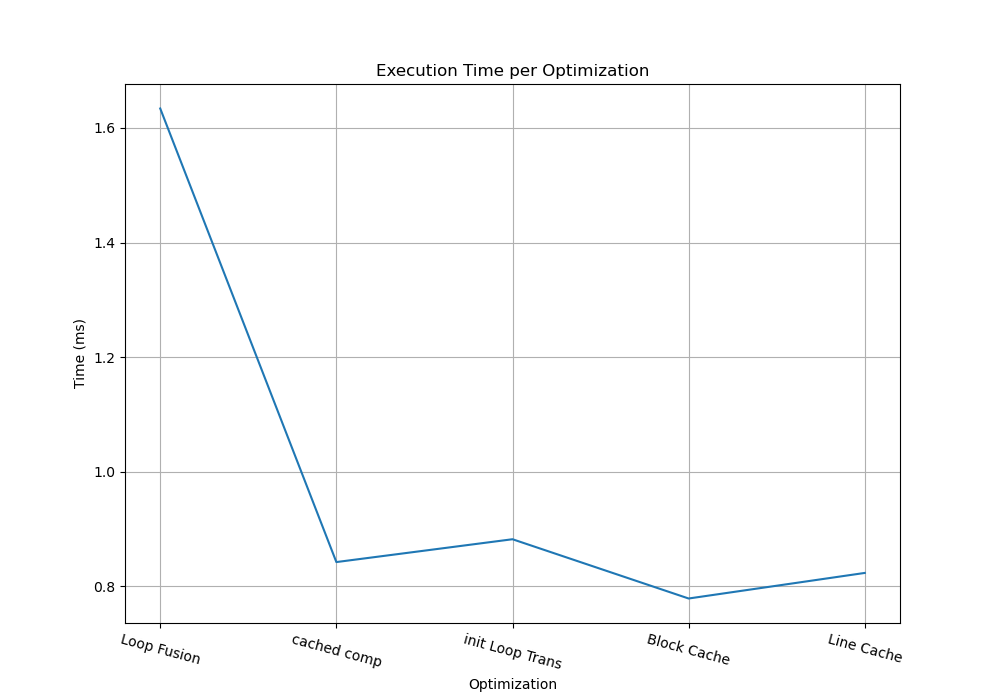
\includegraphics[width=0.6\textwidth]{./plots/measurements.png}
    \caption{Παρουσίαση Μετρήσεων}
    \label{fig:measurements}
\end{figure}
\FloatBarrier

\section{Ερώτημα}

Το \eng{Design Space Exploration} έγινε ``χειροκίνητα'',
λόγω του μικρού χώρου αναζήτησης. Συγκεκριμένα, αφού οι τιμές
των παραμέτρων ήταν $N = M = 10$ και αναζητούνται τιμές του $B$
ώστε να είναι διαιρέτης και των δύο, δοκιμάζονται μόνο οι τιμές
$B = 1$, $B = 2$, $B = 5$ και $B = 10$.

Σε κάθε περίπτωση \eng{buffer}, ο καλύτερος χρόνος λήφθηκε για $B = 5$ και $B = 10$.

\begin{figure}[h]
    \centering
    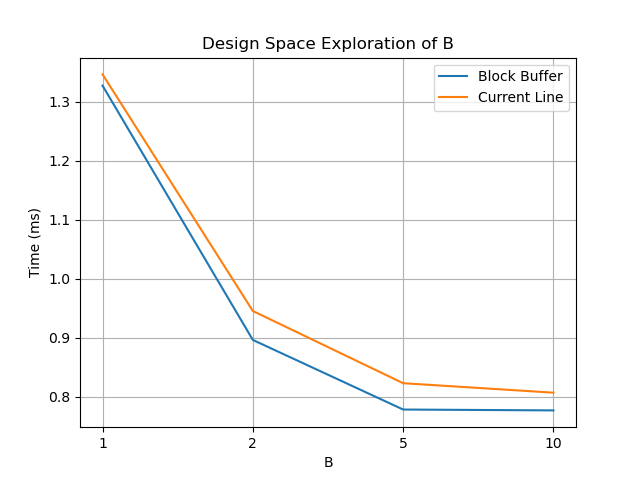
\includegraphics[width=0.6\textwidth]{./plots/dse-b.png}
    \caption{Χρόνοι εκτέλεσης ανά Β}
    \label{fig:dse}
\end{figure}
\FloatBarrier

\section{Ερώτημα}

Στο σχήμα \ref{fig:dse-bxby} φαίνονται οι μετρήσεις για τις διάφορες τιμές των ΒΧ ΒΥ.

\begin{figure}[h]
    \centering
    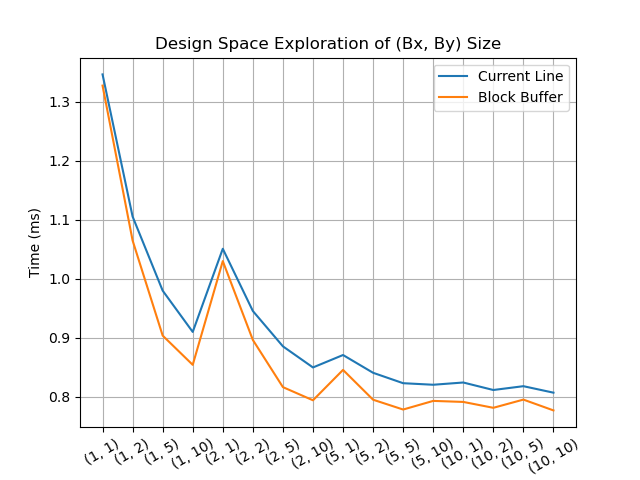
\includegraphics[width=0.6\textwidth]{./plots/dse.png}
    \caption{Χρόνοι εκτέλεσης ανά (ΒΧ, ΒΥ)}
    \label{fig:dse-bxby}
\end{figure}
\FloatBarrier

Γενικά, η τάση είναι να επιταχύνεται η εκτέλεση όσο οι τιμές των Β μεγαλώνουν.
Αλλά, παρατηρείται ότι ο πιο σημαντικός παράγοντας είναι να είναι μεγάλη η 
τιμή του ΒΥ. Αυτό συμβαίνει επειδή ΒΥ είναι το μήκος της γραμμής ακεραίων
η οποία θα αποθηκευτεί σε μία γραμμή της \eng{cache}. Άρα, δεν οφελείται
κανείς έχοντας πολλές γραμμές μικρού μήκους, αλλά οφελείται έχοντας
οσεσδήποτε γραμμές μεγάλους μήκους, αρκεί να χωράνε στην γραμμή
της \eng{cache}. Αυτό θα μπορούσε να είναι ένα καλό κριτήριο.

\clearpage
\part{Παράρτημα}
\selectlanguage{english}
\lstinputlisting[style=CStyle, caption={\eng{final.c}}, label={lst:main}]{./src/hal_entry.c}
\selectlanguage{greek}

\clearpage
\setcounter{section}{0}
\part{Ζητούμενο 2}

\section{Ερώτημα}

\begin{figure}[h]
    \selectlanguage{english}
    \verbatiminput{./text/tables_1.out}
    \selectlanguage{greek}
\end{figure}

\section{Ερώτημα}

\begin{figure}[h]
    \selectlanguage{english}
    \verbatiminput{./text/tables_2.out}
    \selectlanguage{greek}
\end{figure}

Στη δεύτερη αρχιτεκτονική παρατηρείται μείωση των κύκλων. Αυτό είναι κάτι αναμενόμενο αφού αυτή η αρχιτεκτονική διαθέτει \eng{caches} στις οποίες μπορούν να αποθηκευτούν προσωρινά δεδομένα πιο κοντά στον επεξεργαστή.

\section{Ερώτημα}

Οι μετρήσεις παρήχθησαν από τα \eng{bash scripts} \ref{lst:ufs} και \ref{lst:l1}.

\begin{figure}[h]
    \centering
    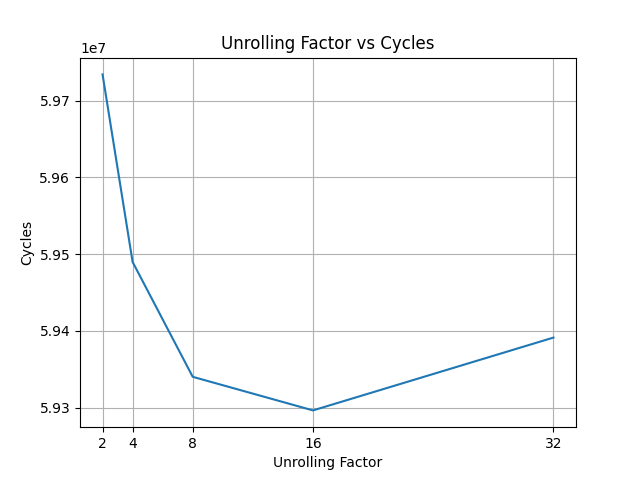
\includegraphics[width=0.8\textwidth]{./plots/unrolling-factor.png}
    \caption{Διάγραμμα μετρήσεων για το \eng{unrolling factor}}
    \label{fig:ufs}
\end{figure}
\FloatBarrier

Από το διάγραμμα παρατηρούμε ότι ο μικρότερος αριθμός κύκλων επιτυγχάνεται με \eng{unrolling factor} ίσο με 16. Για \eng{unrolling factor} ίσο με 32 ο αριθμός κύκλων αυξάνεται. Αυτό συμβαίνει γιατί χαλάει η τοπικότητα λόγω περιορισμένης χωρητικότητας της \eng{cache}.

\begin{figure}[h]
    \centering
    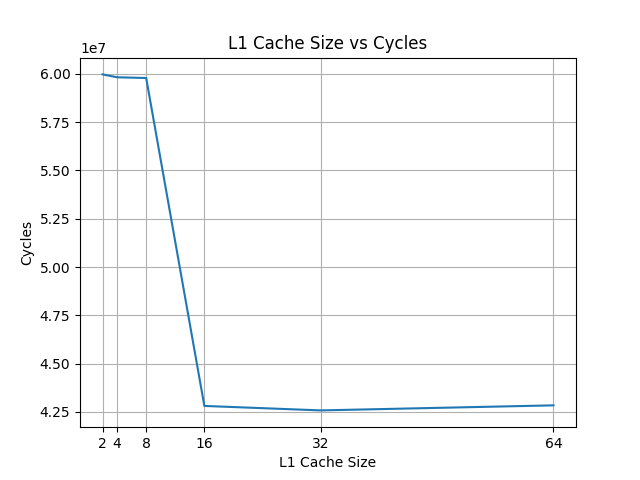
\includegraphics[width=0.8\textwidth]{./plots/l1-cache.png}
    \caption{Διάγραμμα μετρήσεων για το μέγεθος της \eng{L1 cache}}
    \label{fig:l1}
\end{figure}
\FloatBarrier

Παρατηρούμε ότι με αύξηση του μεγέθους της \eng{cache} μειώνονται οι κύκλοι. Ειδικότερα παρατηρούμε δραματική μείωση στη μετάβαση από 8 ΚΒ σε 16 ΚΒ cache size. Από αυτό καταλαβαίνουμε ότι οι απαιτήσεις του προγράμματος σε μνήμη είναι περίπου 16 ΚΒ. Για την ακρίβεια λίγο παραπάνω από 16 ΚΒ αλλά λιγότερο από 32 ΚΒ αφού εκεί δεν παρατηρούμε απότομη μείωση των κύκλων.

\section{Ερώτημα}

Η εξαντλητική αναζήτηση έγινε χρήσει του \eng{bash script} \ref{lst:search} και
το \eng{pareto set / frontier} βρέθηκε με κατάλληλο \eng{python script}
χρήσει της βιβλιοθήκης \eng{pareto}. Τα σημεία του \eng{pareto set} φαίνονται
στο σχήμα \ref{fig:pareto}.

\begin{figure}[h]
    \selectlanguage{english}
    \verbatiminput{./text/pareto.csv}
    \selectlanguage{greek}
    \caption{Οι αρχιτεκτονικές και τα αντίστοιχα \eng{pareto} σημεία}
    \label{fig:pareto}
\end{figure}

Τα δε σημεία από την αναζήτηση του προγράμματος \eng{genOptimizer.py} φαίνονται
στο σχήμα \ref{fig:pareto-genOptimizer}.

\begin{figure}[h]
    \selectlanguage{english}
    \verbatiminput{./text/genOptimizer_PO.csv}
    \selectlanguage{greek}
    \caption{Οι αρχιτεκτονικές και τα αντίστοιχα \eng{pareto} σημεία από το \eng{genOptimizer.py}}
    \label{fig:pareto-genOptimizer}
\end{figure}
\FloatBarrier

Ολοκλήρος ο χώρος αναζήτησης και τα \eng{pareto optimal} σημεία 
φαίνεται στο σχήμα \ref{fig:pareto-space}.

\begin{figure}[h]
    \centering
    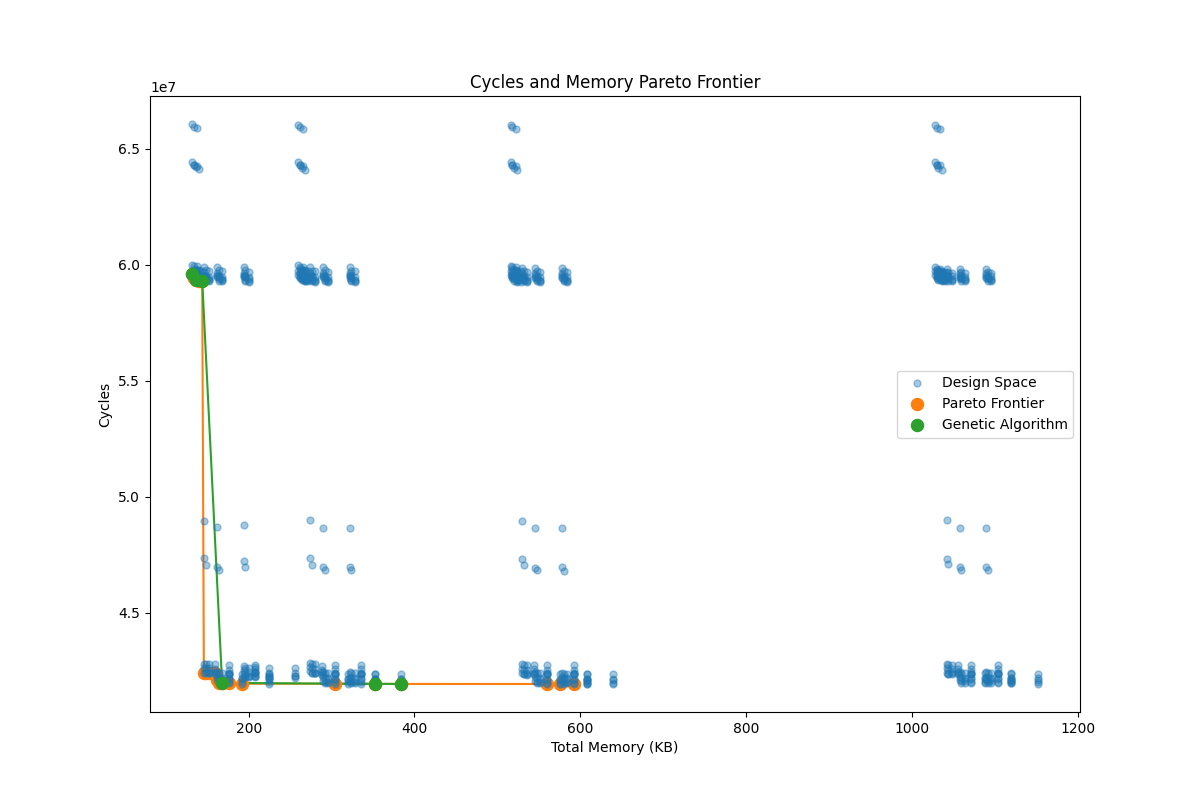
\includegraphics[width=0.8\textwidth]{./plots/pareto.png}
    \caption{Απεικόνιση του χώρου αναζήτησης με το \eng{pareto frontier} επισημασμένο}
    \label{fig:pareto-space}
\end{figure}
\FloatBarrier

\subsection*{Παρατηρήσεις}

Από το Σχήμα \ref{fig:pareto-genOptimizer} βλέπουμε ότι ο γενετικός αλγόριθμος κάνει 6 evaluations, αρκετά λιγότερα συγκριτικά με την εξαντλητική εξερεύνηση του σχήματος \ref{fig:pareto}. Επίσης και ο χρόνος εκτέλεσης είναι σημαντικά μικρότερος. Αυτό συμβαίνει γιατί ο γενετικός αλγόριθμος δεν εκτελεί τις \eng{redundant} περιπτώσεις, δηλαδή τα σημεία στο \eng{Pareto Front} που δεν είναι \eng{Pareto optimal} λύσεις.

Συγκρίνοντας τα δύο \eng{Fronts} διαπιστώνουμε ότι το σωστό είναι αυτό που προκύπτει από την εξαντλητική αναζήτηση (πορτοκαλί) αφού είναι πιο αριστερά στο \eng{plane} άρα τα σημεία του πορτοκαλί \eng{Front} κάνουν \eng{dominate} σημεία του πράσινου \eng{Front}.

\clearpage
\part{Παράρτημα}

\selectlanguage{english}
\lstinputlisting[caption={unrolling-factors.sh}, label={lst:ufs}]{./run-unrolling-factors.sh}
\lstinputlisting[caption={l1-cache.sh}, label={lst:l1}]{./run-l1-cache.sh}
\clearpage
\lstinputlisting[caption={run-search.sh}, label={lst:search}]{./run-search.sh}
\clearpage
\lstinputlisting[caption={pareto-search.py}, label={lst:pareto}]{./exhaustive-search.py}
\selectlanguage{greek}

\end{document}
